\documentclass[10pt,letterpaper,onecolumn,draftclsnofoot,journal]{IEEEtran}
\usepackage[margin=0.75in]{geometry}
\usepackage{listings}
\usepackage{color}
\usepackage{longtable}
\usepackage{graphicx}
\usepackage{PSTricks}
\usepackage{caption}
\usepackage{float}
\usepackage[final]{pdfpages}
\usepackage{tabu}
\usepackage{enumitem}
\usepackage{tikz}

\usetikzlibrary{shapes.geometric, arrows}
\usepackage{courier}
\usepackage[hidelinks]{hyperref}

\setlength{\parindent}{0cm}
\setcounter{secnumdepth}{1}

\newcommand{\namesigdate}[2][6cm]{%
	\begin{tabular}{@{}p{#1}@{}}
		#2 \\[3\normalbaselineskip] \hrule \\[0pt]
		{\small \textit{Signature}} 
		\\[2\normalbaselineskip] \hrule \\[0pt]
		{\small \textit{Date}}
	\end{tabular}
}

\setboolean{@twoside}{false}
\begin{document}
\begin{titlepage}
	\title{The ARLISS Project\\Progress Report\\Senior Capstone}
	\author{Steven Silvers, Paul Minner, Zhaolong Wu, Zachary DeVita\\
		Capstone Group 27\\2016-17 Academic Year}
	\date{\today}
	\maketitle
	\vspace{4cm}
	\begin{abstract}
		\noindent This document details our experiences designing our project over the duration of the academic year. This includes progress made, problems encountered, and plans for the future. We also detail changes we plan to implement in the future.
	\end{abstract}

\end{titlepage}
\tableofcontents
\clearpage

\section{Introduction}
\section{Original Requirements Document}

\includepdf[pages=-]{requirements/srs.pdf}
\section{Changes to Project}
\section{Original Design Document}
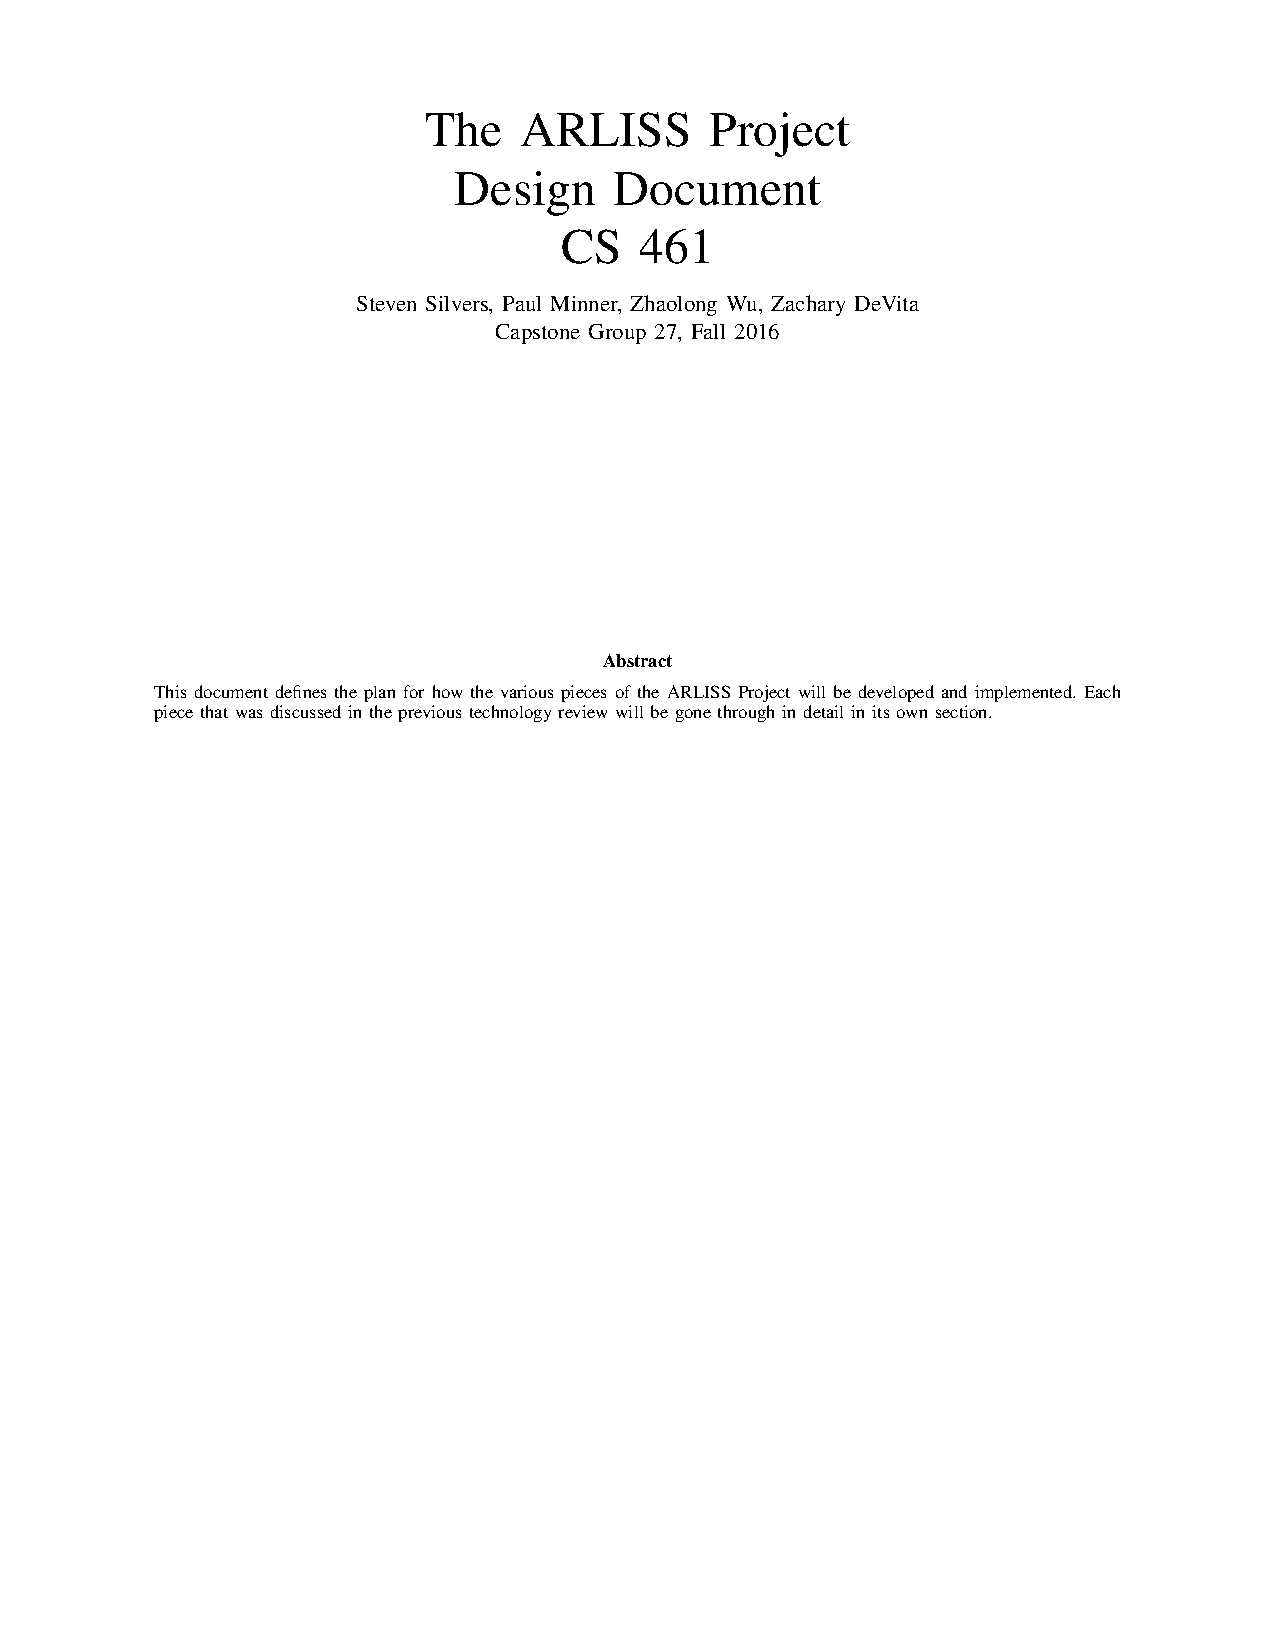
\includepdf[pages=-]{DesignDoc/design.pdf}
\section{Tech Review}

\includepdf[pages=-]{TechReview/tech.pdf}
\section{Weekly Blog Posts}
\section{Poster}
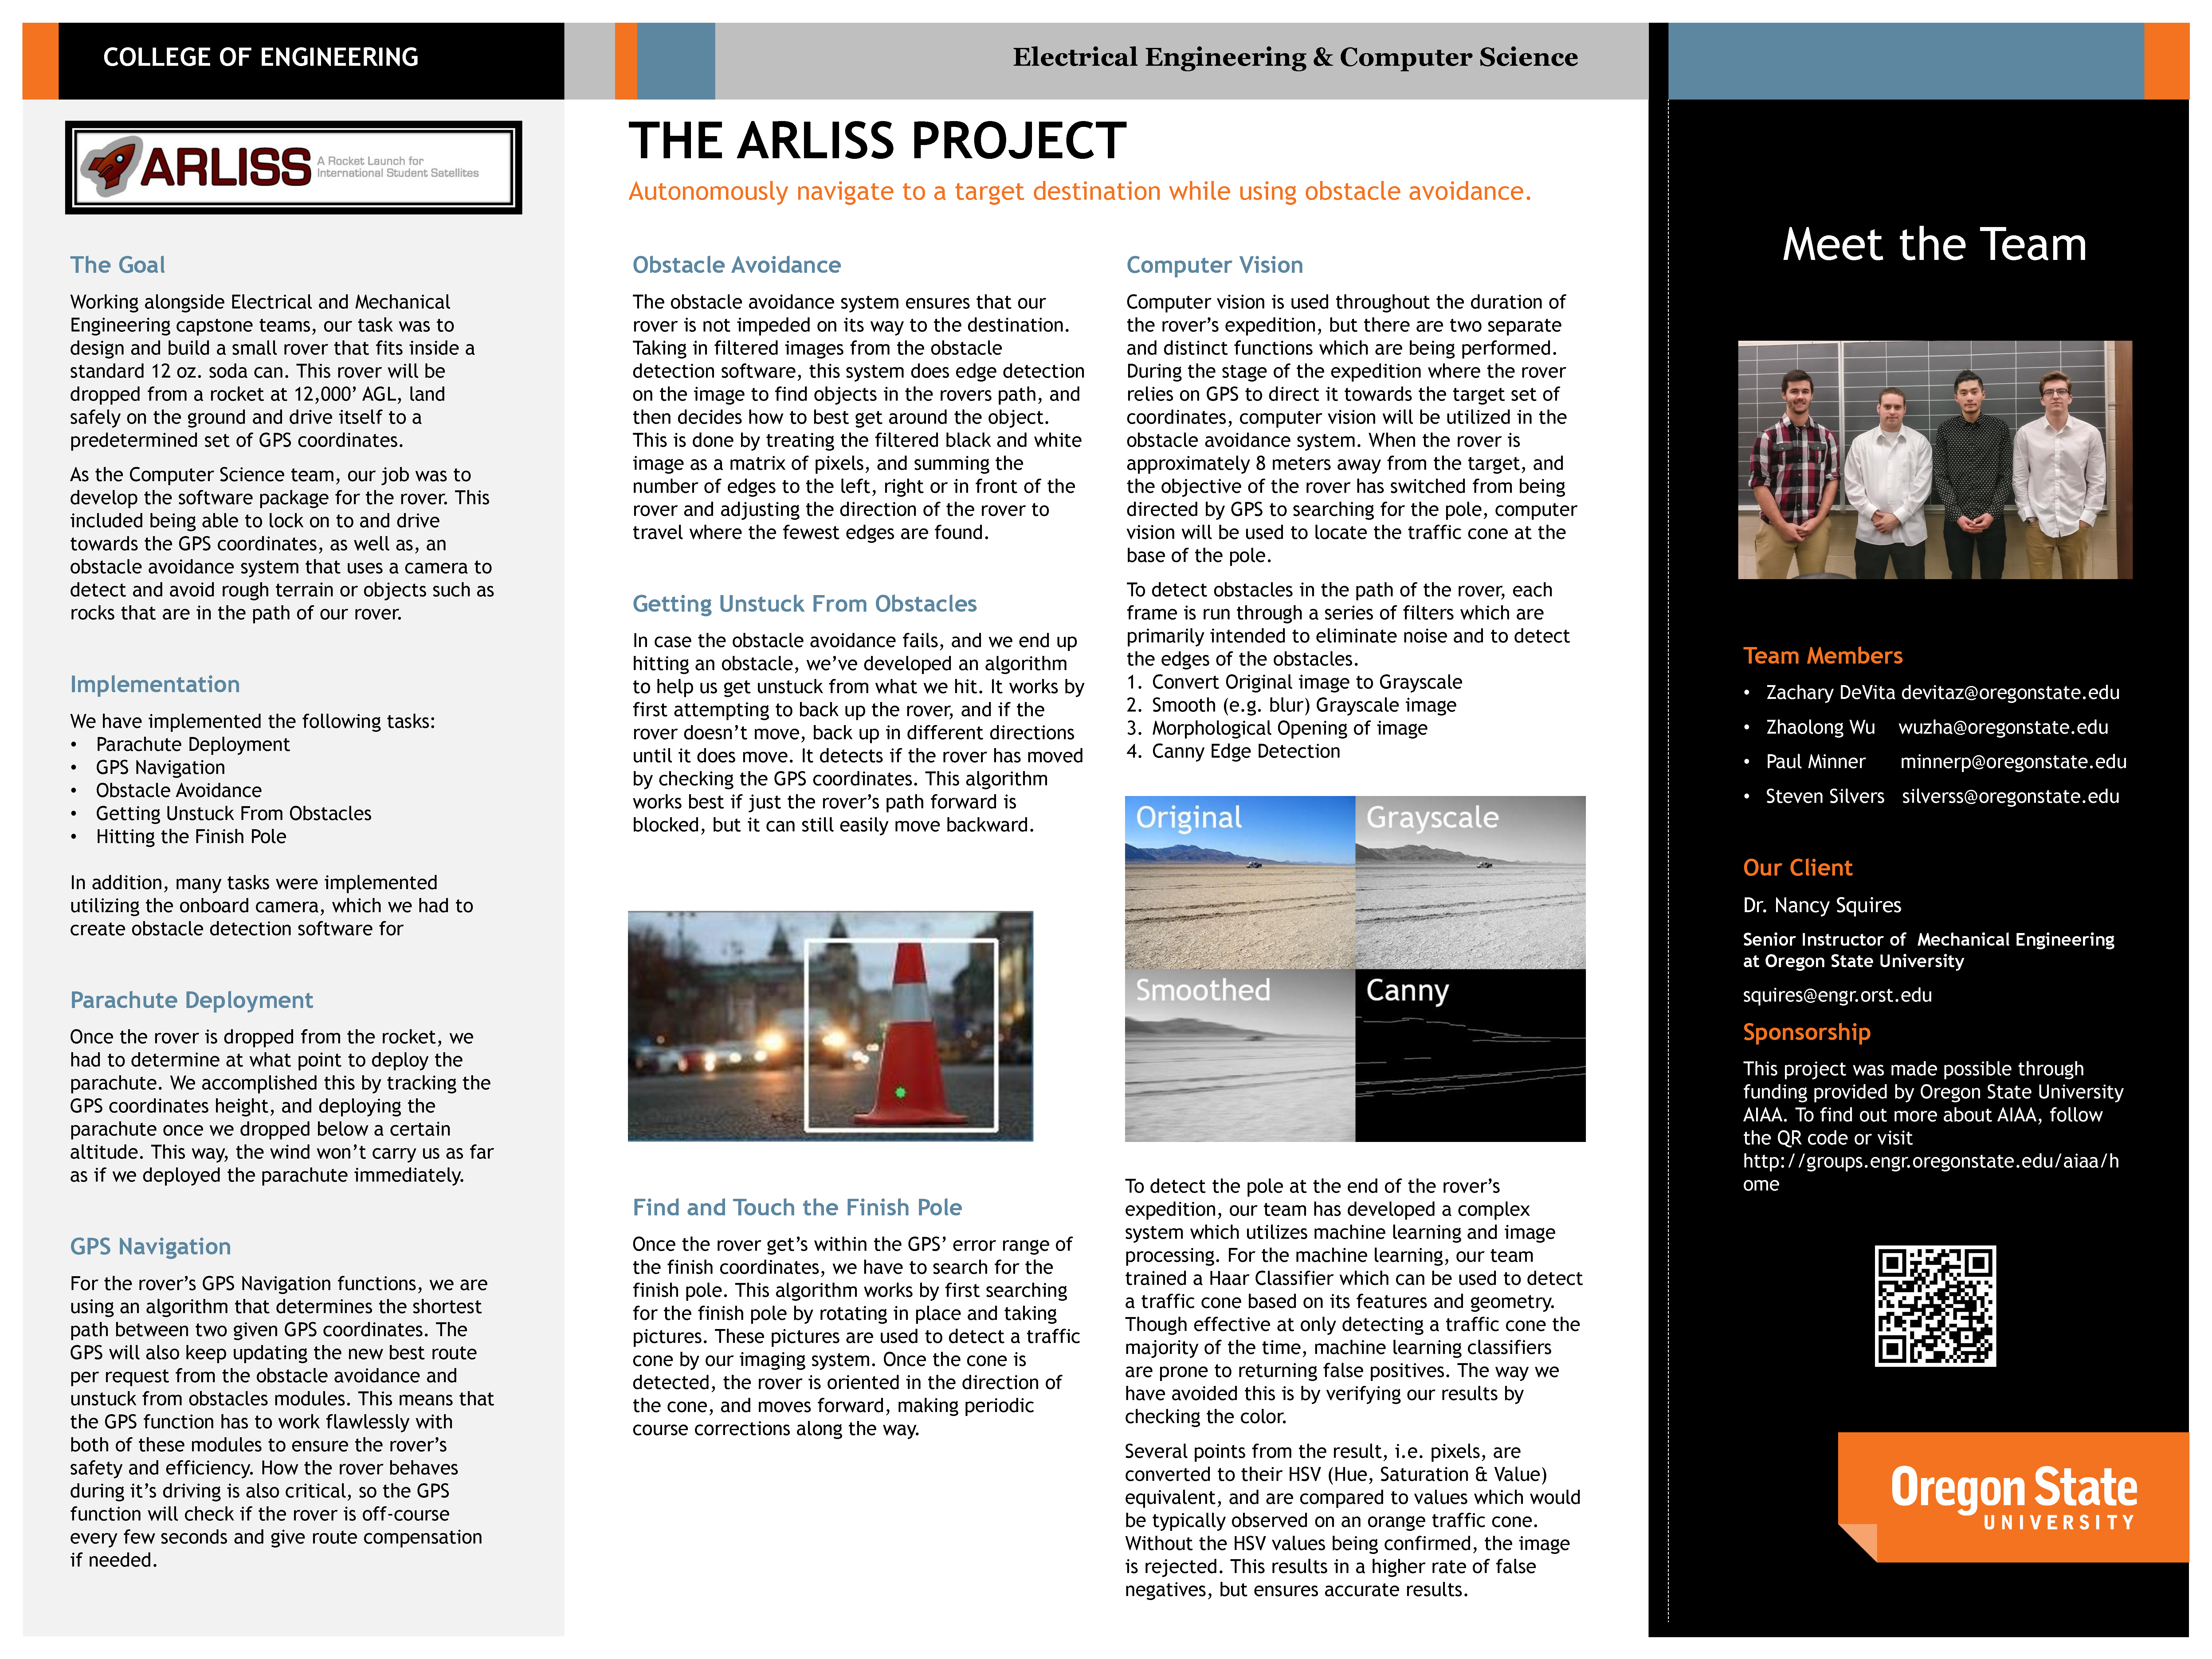
\includepdf[pages=-,angle=270]{Poster.pdf}
\section{Project Documentation}
\section{Learning Sources}
\section{What did we Learn}
\section{Appendix 1: Code Listings}
\section{Appendix 2}

%\section{References}

%\bibliographystyle{IEEEtran}
%\bibliography{tech}

\clearpage

\pagenumbering{gobble}
\vspace{1in}
\noindent \namesigdate{\textbf{Steven Silvers}}
\hfill
\vspace{1in}
\noindent \namesigdate{\textbf{Zhaolong Wu}}
\\
\vspace{1in}
\noindent \namesigdate{\textbf{Paul Minner}}
\hfill
\vspace{1in}
\noindent \namesigdate{\textbf{Zachary DeVita}}
\\
\noindent \namesigdate{\textbf{Nancy Squires}}
\end{document}
